\section{相关工作}
据我们所知，唤醒—睡眠（wake-sleep）算法\cite{hinton1995wake}是文献中另一个适用于同样广泛的连续潜变量模型的在线学习方法。与我们的方法类似，它使用识别模型来近似真实后验。其缺点是必须同时优化两个目标函数，而两者合起来并不对应于对边缘似然或其下界的优化。
唤醒—睡眠算法的一个优点是也适用于离散潜变量模型。它与 AEVB 对每个数据点的计算复杂度相同。

随机变分推断\cite{hoffman2013stochastic}近来受到越来越多的关注。文献\cite{blei2012variational}提出控制变量方法，以降低第\ref{subsec:bound}节所讨论的朴素梯度估计量的高方差，并将其用于后验的指数族近似。文献\cite{ranganath2013black}也引入了降低原始梯度估计量方差的通用方法，即控制变量方法。文献\cite{salimans2013fixedform}在一种高效的随机变分推断算法中采用了与本文类似的重参数化，用于学习指数族近似分布的自然参数。



AEVB 算法揭示了以变分目标训练的有向概率模型与自编码器之间的联系。\emph{线性}自编码器与某类生成式线性高斯模型的联系早已为人所知。文献\cite{roweis1998algorithms}表明，当线性高斯模型的先验为 $p(\bz)=\mathcal{N}(0,\bI)$、条件分布为 $p(\bx|\bz)=\mathcal{N}(\bx;\bW\bz,\epsilon\bI)$，且 $\epsilon$ 趋于无穷小时，PCA 对应于这一特例的最大似然解。

近期关于自编码器的相关研究\cite{vincent2010stacked}表明，无正则化自编码器的训练准则对应于最大化输入 $X$ 与潜在表示 $Z$ 之间互信息的一个下界（参见信息最大化原理\cite{linsker1989application}）。当输入分布固定时，关于参数最大化互信息，等价于最大化负条件熵 $-H(X\mid Z)$。自编码模型下数据的期望对数似然，即负重构误差，是该负条件熵的一个下界\cite{vincent2010stacked}。
然而，众所周知，单靠重构准则本身不足以学到有用的表示\cite{bengio2013representation}。
为使自编码器学到有用的表示，已有多种正则化技术，例如去噪、收缩和稀疏自编码器\cite{bengio2013representation}。SGVB 目标中的正则化项由变分下界决定，例如式\eqref{eq:gaussian_estimator}，因此不需要通常为学到有用表示而引入的额外正则化超参数。
其他相关方法还包括预测稀疏分解（PSD）\cite{koray-psd-08}等编码器—解码器架构，我们也从中获得了一些启发。近期提出的生成随机网络\cite{bengio2013deep}同样相关：其中的含噪自编码器学习一个马尔可夫链的转移算子，该链从数据分布采样。文献\cite{salakhutdinov2010efficient}则利用识别模型提高深度玻尔兹曼机的学习效率。
这些方法要么针对未归一化模型，即玻尔兹曼机等无向模型，要么仅限于稀疏编码模型；而我们提出的算法用于学习一大类有向概率模型。

近期提出的 DARN 方法\cite{gregor2013deep}也通过自编码结构学习有向概率模型，但其方法适用于二值潜变量。
更近的工作\cite{rezende2014stochastic}也利用本文所述的重参数化技巧，将自编码器、有向概率模型和随机变分推断联系起来。他们的工作独立于我们开展，为 AEVB 提供了另一个视角。





\begin{figure}[t]
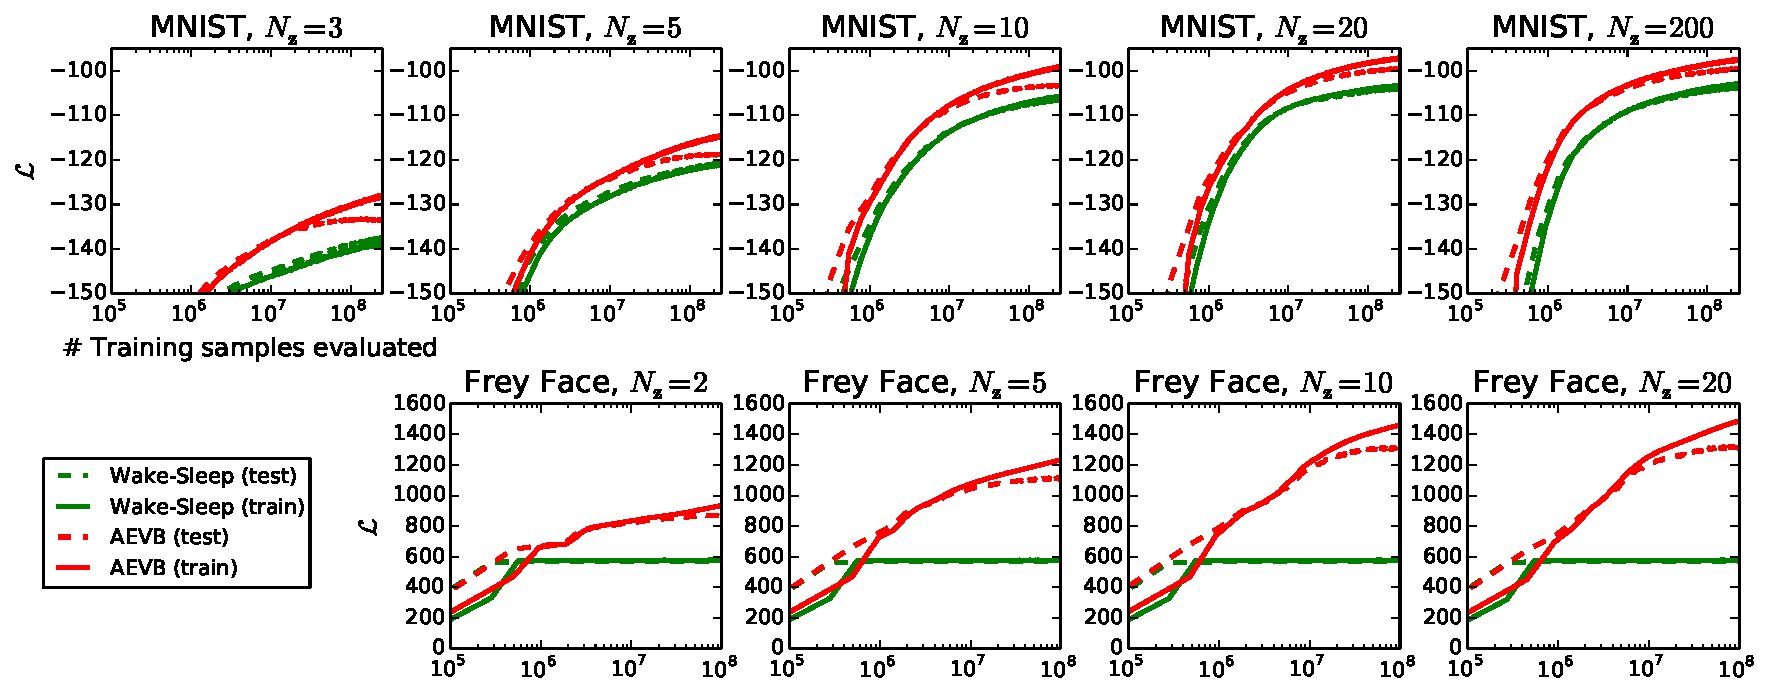
\includegraphics[width=0.95\columnwidth]{assets/figures/graph_lowbound.pdf}
\caption{在不同潜在空间维数 $N_{\bz}$ 下，比较 AEVB 与唤醒—睡眠算法对下界的优化效果。在所有实验中，我们的方法收敛都明显更快，且得到更好的解。有趣的是，增加潜变量并未加重过拟合，这可以用下界的正则化作用来解释。纵轴为估计的每个数据点的平均变分下界；估计量方差很小（$<1$），故未绘出。横轴为累计评估的训练数据点数。在有效运算速度为 40 GFLOPS 的 Intel Xeon CPU 上，每处理一百万个训练样本约需 20--40 分钟。}\label{fig:lowbound}
\end{figure}
